%! TEX root = ../main.tex
% =============================================================
% IMMUTABLE — generated automatically, do not edit this block
%   script          : analysis_scratch/parallel_probe_agreement.py
%   plot_type       : parallel_probe_agreement
%   chapter         : 04
%   threshold       : 10%
%   n_runs          : 78
%   n_consistent    : 62
% =============================================================
\begin{figure}[htbp]
  \centering
  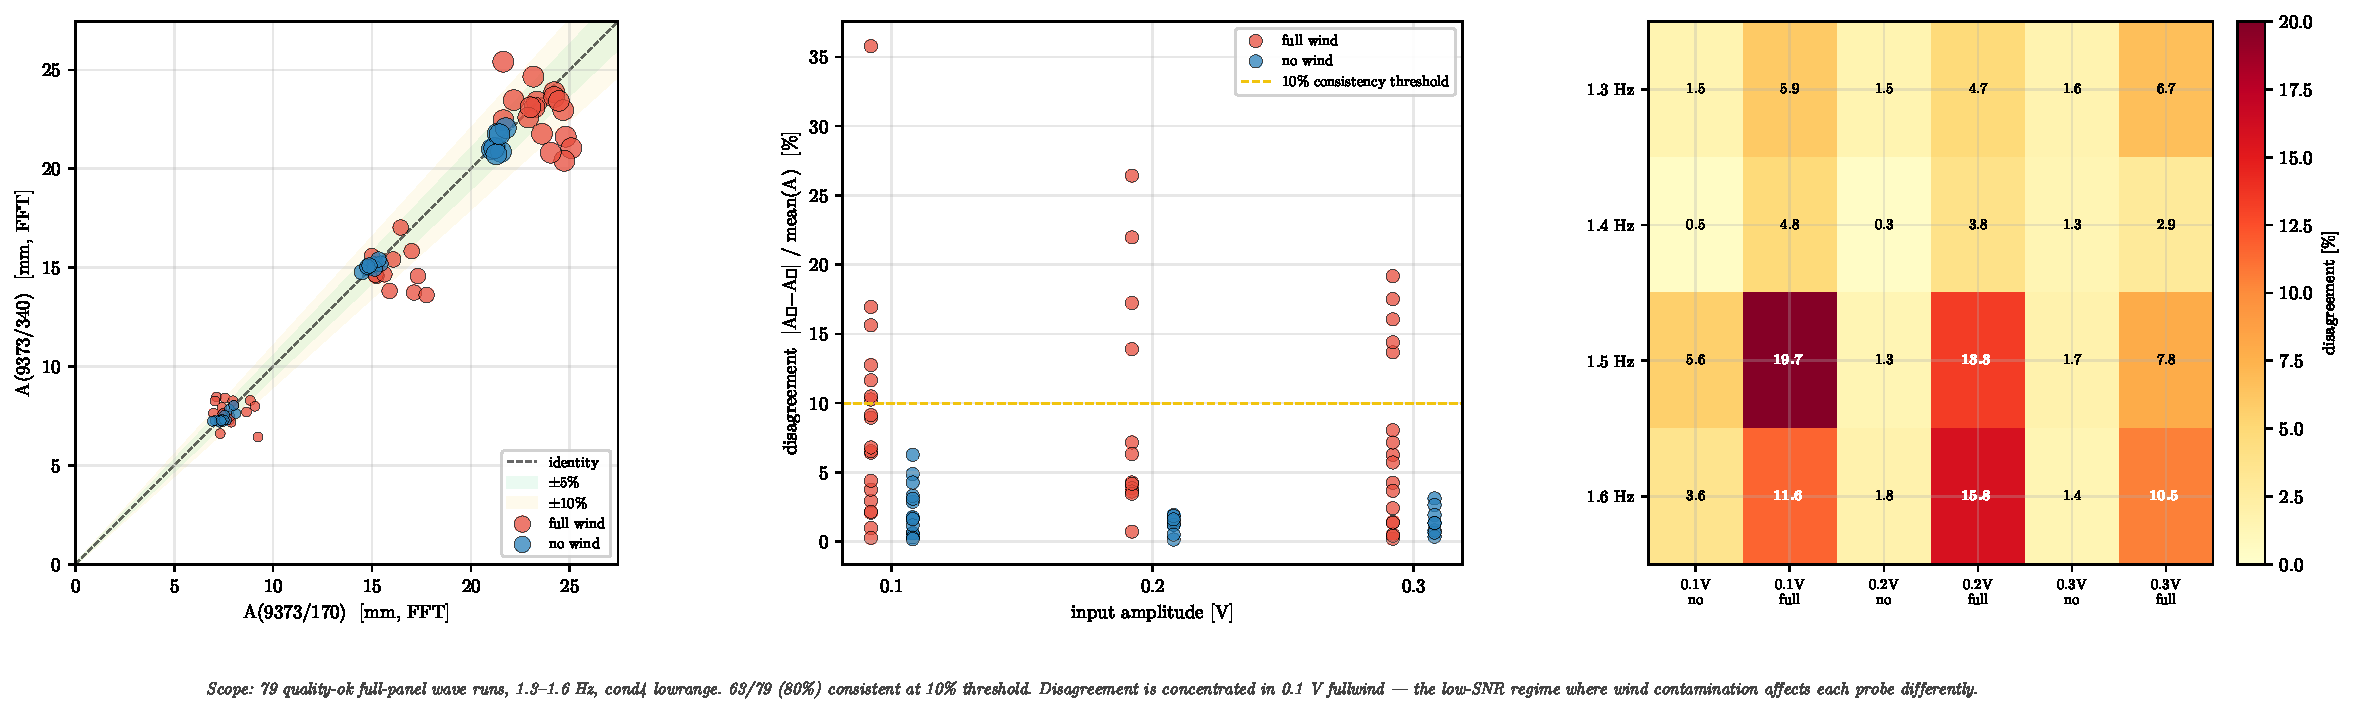
\includegraphics[width=0.98\linewidth]{FIGURES/ch04_parallel_probe_agreement.pdf}
  \caption[Parallel-probe agreement]{%
    Parallel-probe cross-check for the canonical IN reference. 9373/170 and 9373/340 sit at the same longitudinal distance from the paddle; in a 1D-wave approximation they should see the same incident amplitude. (a) A(9373/170) vs A(9373/340), identity line and $\pm 5$/$\pm 10$\% bands. Colour: wind; marker size: input amplitude. (b) Fractional disagreement versus input voltage, split by wind. The $10\%$ consistency threshold is drawn; disagreement is concentrated at $0.1$\,V fullwind (low SNR, wind contamination dominates the IN probe FFT). (c) Heatmap of mean disagreement per (frequency, amplitude, wind) across the thesis band. Across all 78 quality-ok full-panel wave runs in the thesis scope (1.3--1.6\,Hz, cond4 lowrange), $62/78$ ($\sim79\%$) are within the $10\%$ threshold. This validates replacing the single-probe IN reference with the mean of both 9373 probes as the canonical IN amplitude in all CH05 figures.
  }
  \label{fig:ch04_parallel_probe_agreement}
\end{figure}
